\section{TRI-D Interferometric imaging}\seclab{Intf}

Interferometry can be performed working only with the signals measured in the antennas, i.e.\ without unfolding the antenna function, and is referred to as Signal Interferometry (SI), which is by now considered obsolete. This because the method has many unsolved issues with signs due to the antenna function and the emission pattern being angle dependent. More sophisticated is to convert the measured signal in the X- and Y- dipoles to the radiation electric field at the antenna and use this for interferometry, presently the preferred and only option. This will be named E-field Interferometry (EI) when it needs to be contrasted with SI.

Source finding is performed by the script \verb!"Interferometry.sh"! residing in the FlashFolder. The running of the script is controlled by \verb!"Interferometry.in"!, which typically resembles:

\begin{linenumbers}
\resetlinenumber
\tiny
\begin{verbatim}
 &Parameters  RunOption= "TRI-D"
 OutFileLabel= "XYZ"
 AntennaRange= 100.     ! Maximum distance (from the core) for the range of the antennas (in [km]).
 TimeBase=320.    ! Time-offset from the start of the data, best if kept the same for all analyses for this flash
! Simulation= ""     ! Run on simulated data from such files.
! ChainRun= 0     ! Automatically start jobs (for - previous or + following timeslots, made to follow a negative leader.
! IntfSmoothWin= 19     ! Width (in samples) of the slices for TRI-D imaging.
! PixPowOpt= 0     ! =0=default: Intensity=sum two transverse polarizations only; =1: Intensity=sum all polarizations weighted with alpha == intensity of F vector; =2: Intensity=sum all three polarizations, including longitudinal with the full weight
! CalibratedOnly= T     ! Use only antennas that have been calibrated.
 NoiseLevel= 1.0000000000000000E-002     ! Any weaker sources will not be imaged.
 Calibrations="Calibrations202202071332.dat" ! FldCal all antennas
 BadAnt_SAI=   5095,   7093,  11089,  13088,  13089,  17084,  17085,  17094,  17095
               101085, 141083, 141086, 141087, 167094, 169082, 169090, 169094,
 ExcludedStat=  "RS305"      ! Mnemonics of the stations that should be excluded.
 SignFlp_SAI=  142092, 142093
 SaturatedSamplesMax= 3     ! Maximum number of saturates time-samples per chunk of data
 &end  !
S  231.  8.2 ,-3.7, -34.11    !    Reference/Source-| time, & position
C   80 2.5, 30 2.5, 72 4 !   Polar(Phi,Th,R)/Carthesian(N,E,h) | 3x(#gridpoints, grid spacing)
F  25000  15000 10.   !  First/Median| SumStrt, SumWindw, AmpltPlot
\end{verbatim}
\end{linenumbers}

The lines in the namelist \verb!"&Parameters"! input specify:
\begin{enumerate*}
\item \verb!RunOption= "TRI-D"!: Run the TRI-D Imager
\item \verb!OutFileLabel="XYZ"!: Additional label used for the output files, including the plots.
\item \verb!AntennaRange=100.!: The maximal distance (in [km]) from the reference station of the antenna stations that are included in imaging.
\item \verb!TimeBase=320.!: This time is added to the relative time specified in the input.
\item \verb# Simulation= ""#: No simulated data are used in blank, otherwise the simulated data are read from these files and should have the same value as used when generating the simulated data, see \secref{Sim}.
\item \verb# ChainRun=0# (Integer, default=0): If =0 the present run will not spawn any children, otherwise see \secref{ChainRun}.
\item \verb!IntfSmoothWin=19! (Integer, default=20): the width of the sampling function used for Time Resolved Imaging (in [samples]). This number should be of the order of the impulse-response time, about 20~samples.
\item \verb!PixPowOpt=! (Integer, 0): selects how the intensity of a pixel is calcula
   \\\verb!PixPowOpt =0! (default): sum two transverse (as seen from the core) polarizations only.
   \\\verb!PixPowOpt =1! : sum all polarizations weighted with alpha to compensate $A^{-1}$ thus intensity =  $|\vec{F}|$, see \eqref{F_as}.
   \\\verb!PixPowOpt =2! : Sum all three polarizations, thus including longitudinal with the full weight.
\item \verb!CalibratedOnly= T! (logical, .true.): use only antennas that have been calibrated.
\item \verb!NoiseLevel=!: only sources with a coherent intensity exceeding this value will be imaged.
\item \verb!Calibrations =""!: The name of the file containing calibration data.
\item \verb!"BadAnt_SAI="!: These antennas are excluded from the analysis.
\item \verb!"SignFlp_SAI="!: The amplitude for this antenna is multiplied by minus unity.
\item \verb!"ExcludedStat="!: Mnemonics of the stations that will be excluded from interferometry. The exclusion is usually based on unexpected phases.
\end{enumerate*}


The following lines specify:
\begin{enumerate*}
\item[line +1:]   ``\verb#S  231.  8.2 ,-3.7, -34.11#''
   \begin{enumerate*}
   \item[1] Option, "R" or "S" (capital, the very first character on this line): time is specified at the Reference antenna or at the Source location for the tesseract.
   \item[2] $t_t$, the starting time of the data-chunk in which the tesseract is taken, given in time [ms]. Time is taken relative to \verb!"TimeBase"!.
   \item[3-5] Space coordinates of the center of this tesseract, in (N,E,h) notation. The units may be [km] or in [m], but have to be the same for all three.
   \end{enumerate*}
\item[line +2:]   ``\verb#C   80 2.5, 30 2.5, 72 4#''
   \begin{enumerate}
   \item[1] Option, "P" or "C" (capital, the very first character on this line): determines if a Polar or Cartesian grid is used for the tesseract. The polar grid is taken as a wedge, focussed ar the reference antenna. A Polar grid is specified in the order: Azimuth angle $\phi$, elevation angle $\theta_e$, and distance to reference antenna $R$. A Cartesian grid as: Northing $N$, Easting $E$, and altitude $h$.
   \item[2, 4, 6] Number of grid points, counting from the center.
   \item[3, 5, 7] Grid spacing in degrees or meter.
   \end{enumerate}
\item[line +3]:   ``\verb#F  25000  15000 10.#''
   \item[1] Option, ``F" or ``M" (capital, the very first character on this line): determines if the time is set at the First or the Middle sample of the time window.
   \item[2] (integer): Time-offset of the tesseract from the start of the data chunk, in samples of 5 ns. Care should be taken that the start of the tesseract is at least 1000 samples from the beginning of the data chunk to avoid antennas from dropping out. Error messages are generated and image is truncated when the value is too small. If option ``F" (``M") is specified the value is pointing to the First (Middle) time sample of tesseract.
   \item[3] (integer): The length of the window (in [samples]) that is imaged. The maximum window length is 60k~samples (corresponding to 0.3~ms) to which 40 (=$2\times$"IntfSmoothWin") may be added is to accommodate for the beginning and end smoothing windows when performing Time Resolved Imaging (see \secref{TRID}).
   \item[4] : an indicator of the maximum size of the circles used in plotting, taken proportional to source intensity. If negative, dots are used and the intensity spectrum is not analyzed.
\end{enumerate*}


This script produces TRI-D images (see \secref{TRID} for the procedures followed)
and puts the results in several data files in the subdirectory \verb!"files"!. It also prepares the command files (in \verb!"GLE-plotsXYZ.sh"!) for running the GLE scripts \cite{GLE} to produce \verb!"InterfContourXYZ.pdf"!, \verb!"XYZInfImgBar_0.pdf"!, \verb!"XYZInfImaMx_0.pdf"!, \verb!"InterfTrackXYZ.pdf"!. The interferometric hypercube is also shown in the plot of the source locations.

It is recommended to subsequently run the script \verb!"DataSelect.sh"! using \verb!"DataSelect.in"! as input to produce the plots that are zoomed in on the region of interest, see \secref{DataSelect}

\subsection{Chainrun} \seclab{ChainRun}

If \verb# ChainRun=0# the present run will not spawn any children, otherwise, a chain of jobs will be generated to allow for the TRI-D imager to follow the track of a leader, or to image a fixed spot for a long time period.
if \verb# ChainRun=0# is non zero line ``+1'' may have a different structure which is determining what the structure of the chaining will be.

Typically [line +1] may read:  ``\verb#S  825.15   "I-19A-1b-D3a.trc" #'' where the space coordinates have been replaced by a file name containing a track. The first few lines of this file could read
{\tiny
\begin{verbatim}
   825.0   -12.  -27.05   7.6
   826.12   -12.  -27.05   7.6
  826.12049     -11.872760     -26.808671      7.4762350
  826.13483     -11.822525     -26.901188      7.5054529
  826.14391     -11.817934     -26.985353      7.4927362
\end{verbatim}
}
where the bulk of the file was generated using the 'longtrack' option in utility \verb!DataSelect! as described in \secref{DataSelect}. Each line gives the coordinates of the track as (time, N, E, h). The file may also be a .dat file (in stead of .trc),  having the same format at image-source files, i.e.\ (label, t, x, y, z). The program will construct a cube of size as specified in [line +2] centered at the the position on the track at time $t_t$=825.15 for the present example. At the end of the run an input for a following job is created where the time on the track is increased by the time duration of the tesseract. \verb# ChainRun# will be decreased by one and a new job is submitted. This proceeds till \verb# ChainRun# is reduced to zero, or the end of the track is reached. The present value of \verb!"ChainRun"! is worked into \verb!"OutFileLabel"! as well as the naming of the spawned scripts.

When \verb# ChainRun# is negative, the time of the next run will be decreased and \verb# ChainRun# is increased, i.e.\ the track is scanned in the opposite direction as before. 

In case not a track, but coordinates are given, the program will center the new image cube at the center of intensity of the present image. This option sounds fancy but in practice does not really perform up to expectation.

If the track file name is followed by a positive real, this is interpreted at the time on the track. The tesseracts will follow the track in space coordinates, but are all taken at the same fixed time given by $t_t$. The next image box is now taken such that the side touches that of the previous, independent of the time duration of the tesseract, but following the track. This option is used in Ref.~\cite{Scholten:2023PL}. 

\subsection{Output}\seclab{Interf}

The produced .dat files are plain text files and contain some header lines with some general information followed by the specific data of the sources that are found and pass some very crude criteria. The files have a format that is suitable for the plotting script \verb!"SourcesPlot.gle"!. The naming of these data files is as in \verb!"XYZIntfSpecPowMx_d.dat"!, where \verb!"XYZ"! is set by the user through \verb!"OutFileLabel=XYZ"! when running the interferometry option; \verb!"IntfSpecPow"! is fixed for these kind of files; \verb!"Mx"! implies that these source positions were determined using the quadratic maximum search while for \verb!"Bar"! the, by now obsolete, barycentric procedure was used, see \secref{Max}.
This file also contains the coordinates of the corners of the hypercube used in the interferometry calculation.


\subsubsection{Intensity plot}

\begin{figure}[th]
\centering{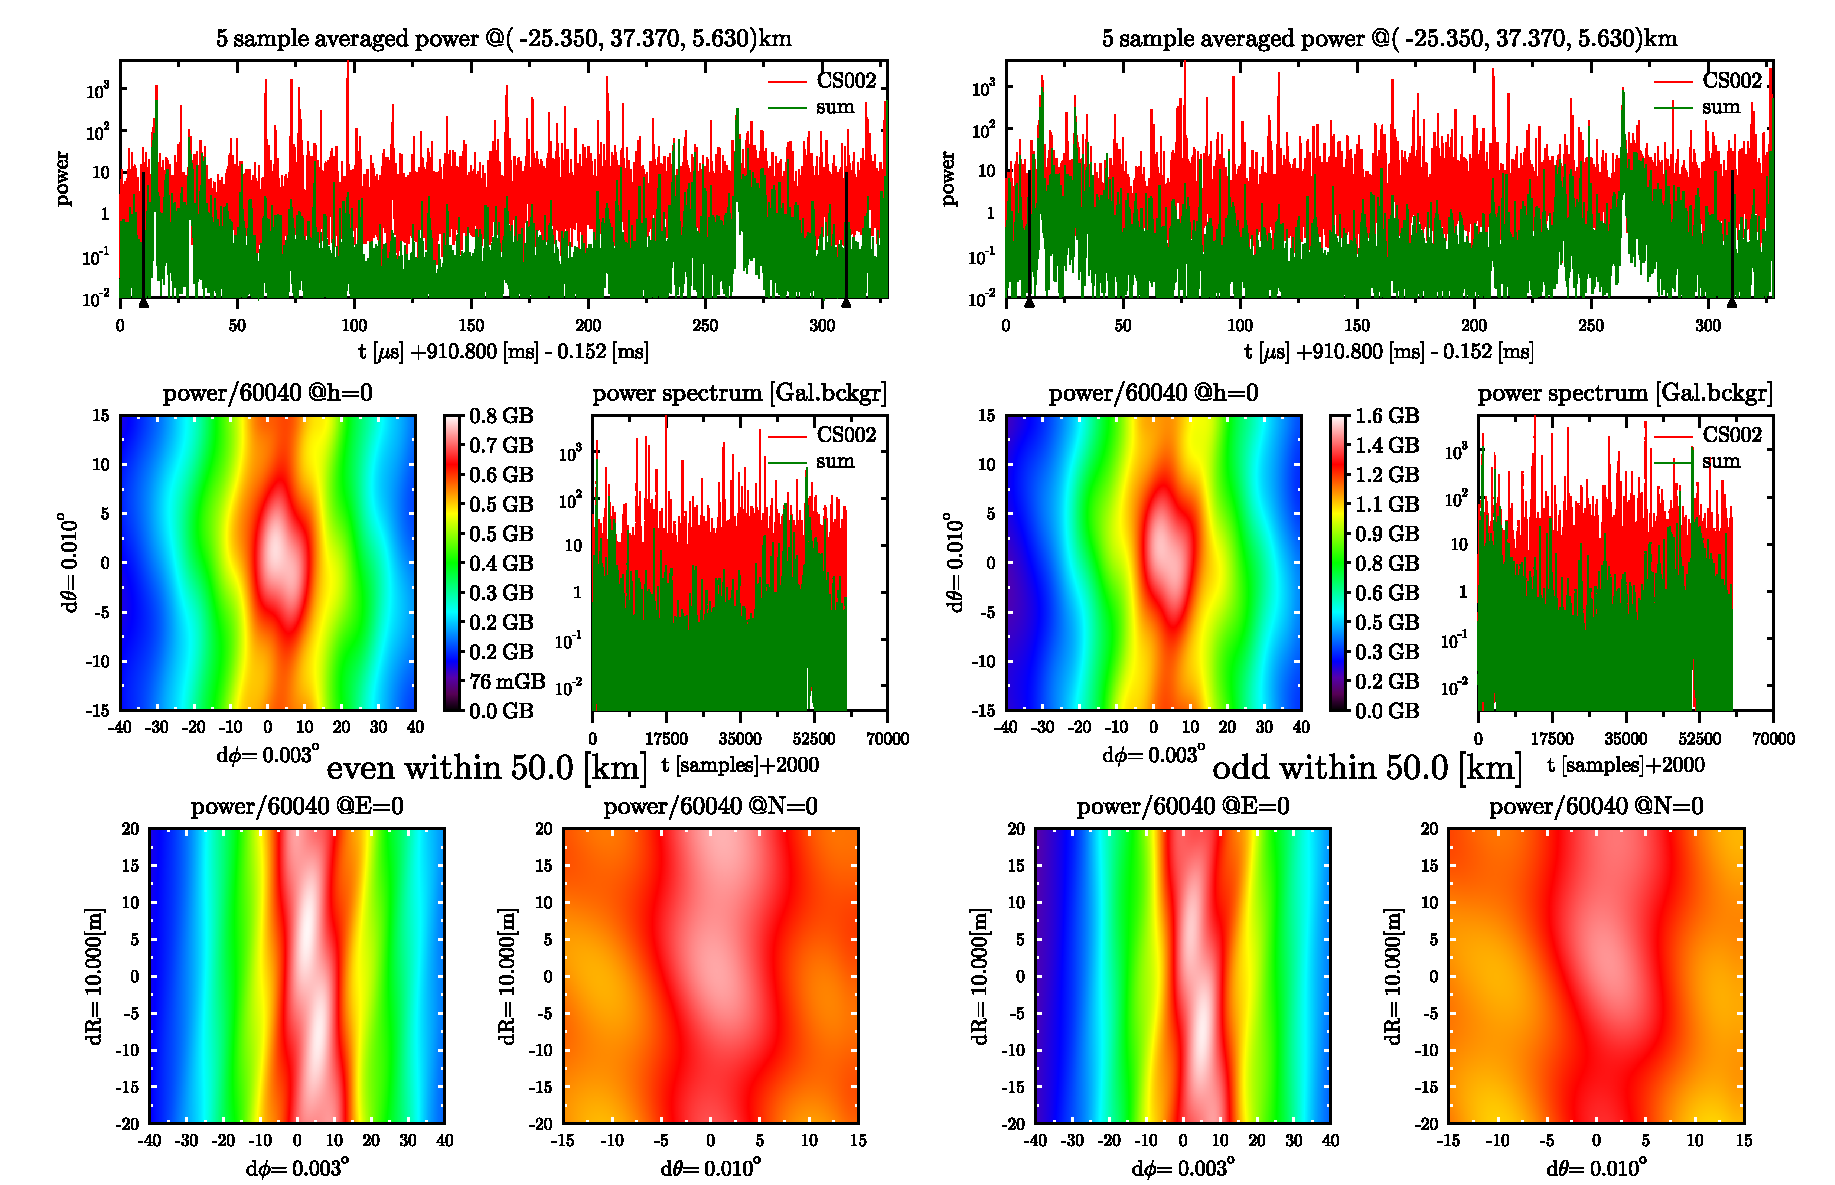
\includegraphics[width=0.99\textwidth]{Figs/InterfContourSE20A7-Np-} }
%\centering{\includegraphics[ bb=1.0cm 2.4cm 24.5cm 25.7cm,clip, width=0.49\textwidth]{../Figs/SE20A7-NPMx_1HIntfSpecSel} }
	\caption{Typical image for the TRID Imager as created by running ``InterfSrcSel.sh".}	 \figlab{TRIDIntImg}
\end{figure}

A typical interferometric Intensity plot is shown in \figref{TRIDIntImg}. These are produced separately for even- (left side of \figref{TRIDIntImg}) and odd- (right side) numbered antennas. The top shows in red the spectrum in the reference antenna while green shows the coherent sum of all antennas in the field, beamed towards the central pixel of the hypercube. The green spectrum is normalized by the number of antennas ($N_a$, i.e.\ the geen and red should fall on top of each other if the signal would be completely coherent for this direction. If the signal is random noise it should be at a fraction of 1/$N_a$. This signal power is rebinned over 5 samples. With black lines the zoom-in window is indicated. The zoomed-in spectrum is shown below it, using the same convention but without re-sampling. The other figures show the intensity along a plane through the hypercube, top left at dR=0, the bottom two at $d\theta=0$ and $d\phi=0$. Step sizes and ranges are specified in the input line starting with `P'.

\begin{figure}[th]
\centering{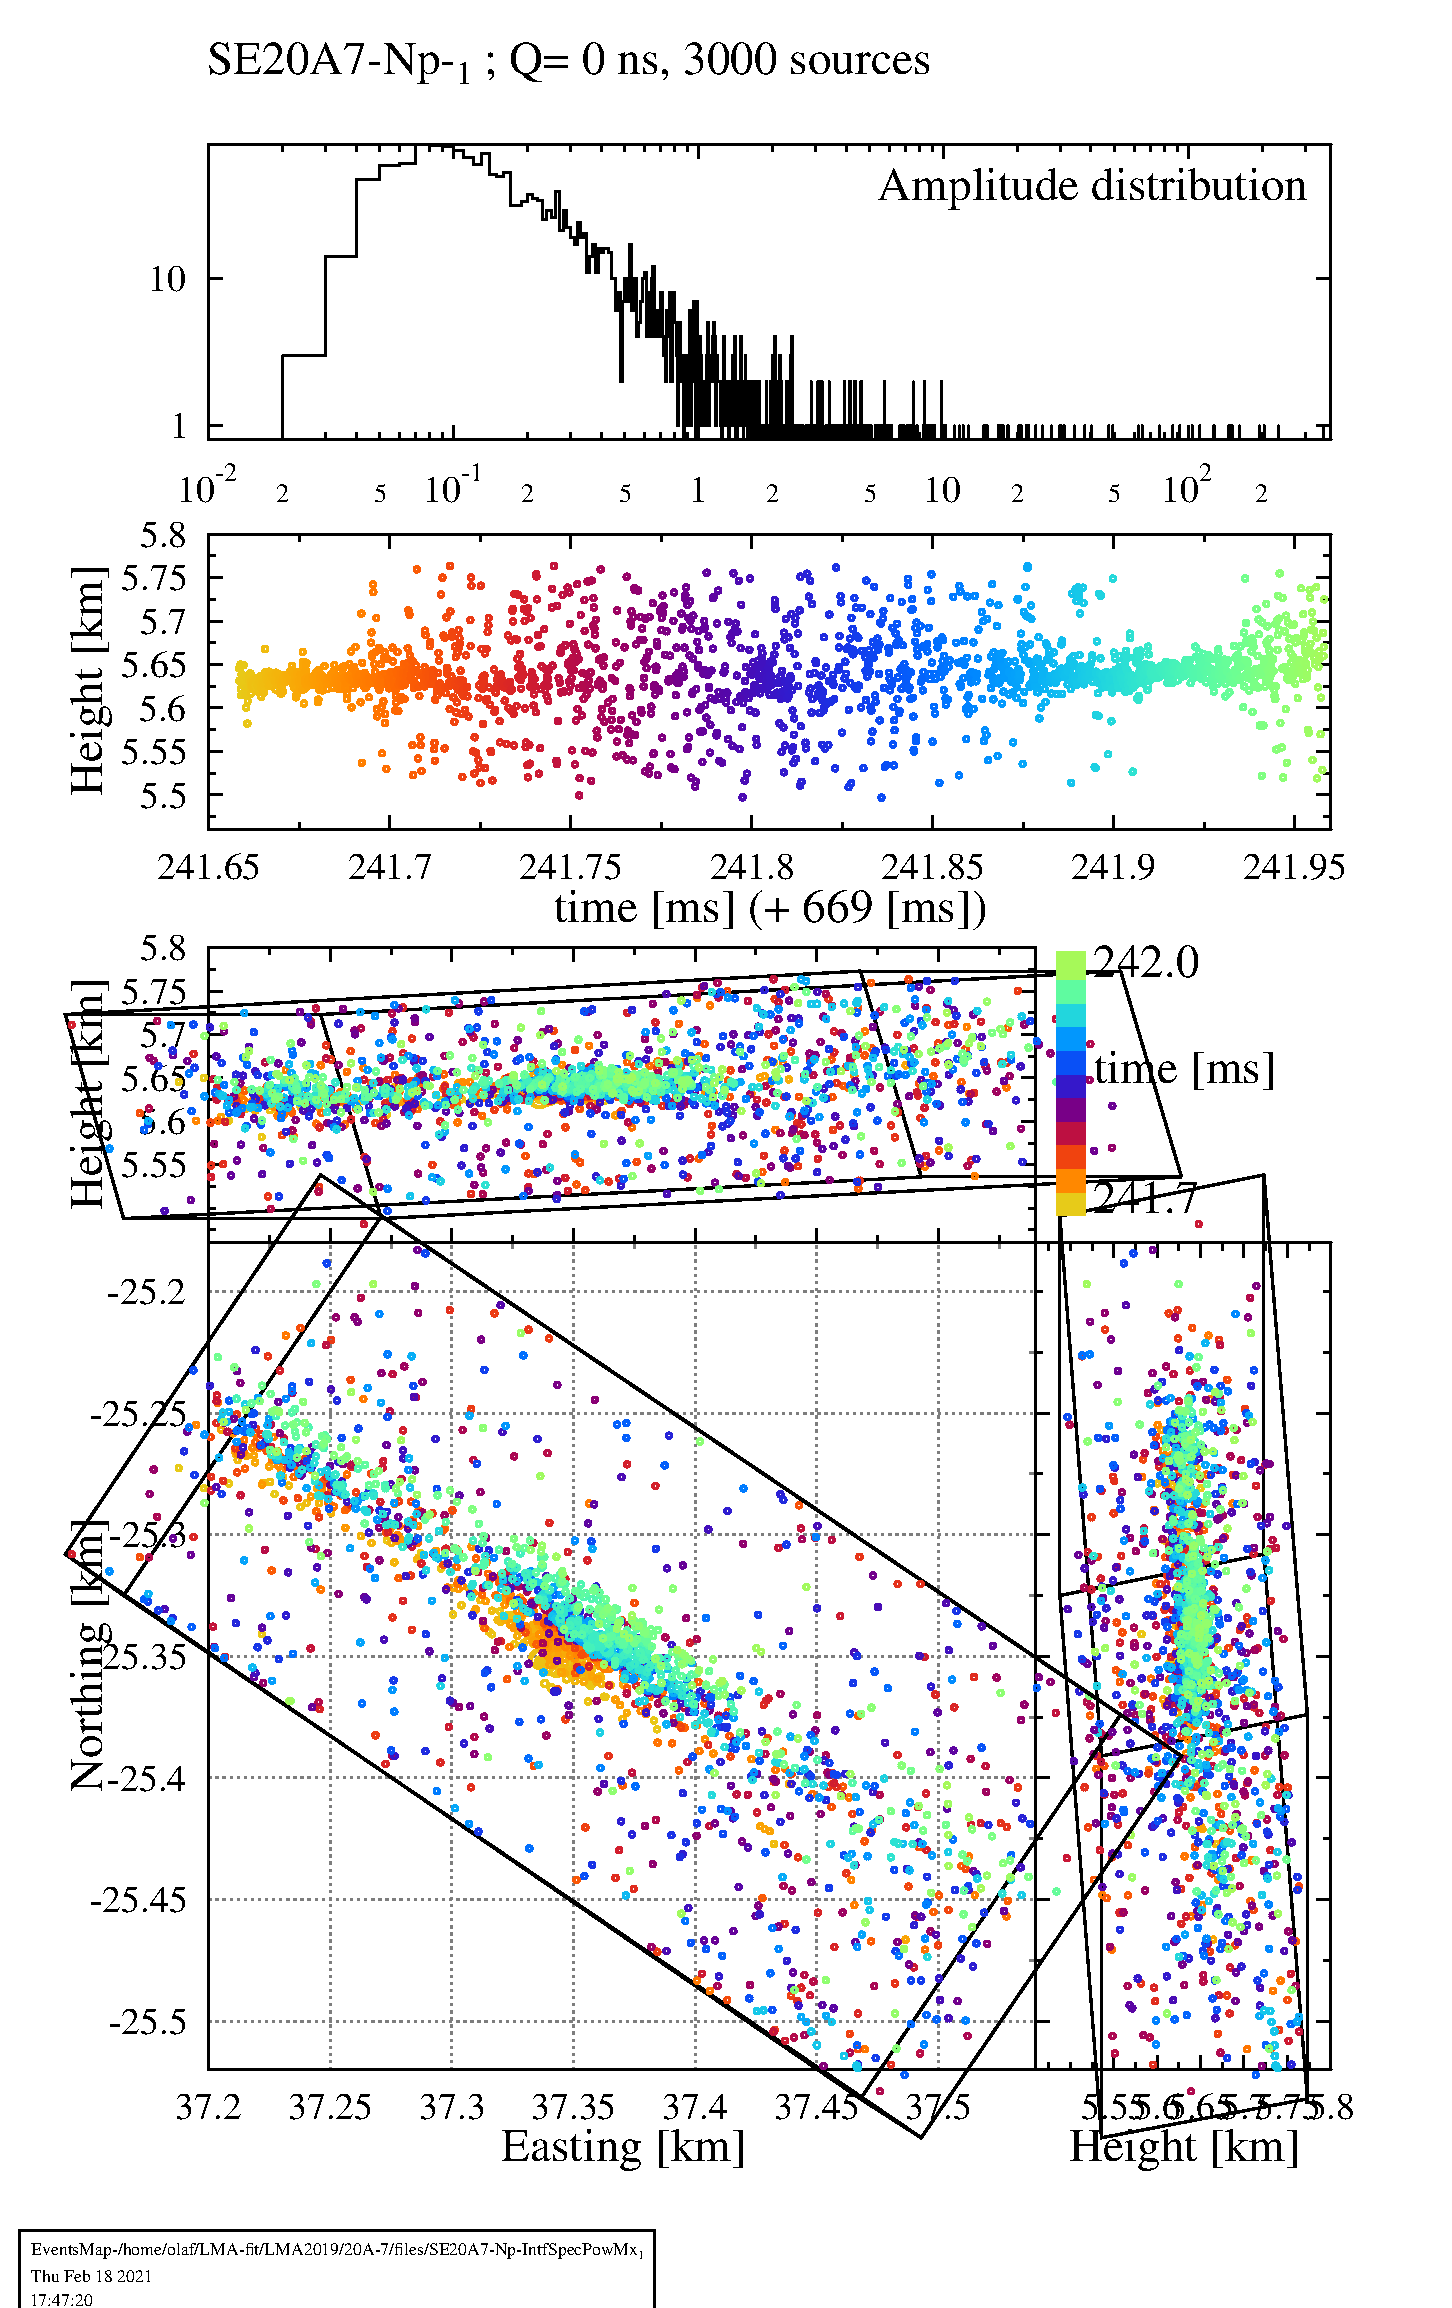
\includegraphics[width=0.49\textwidth]{Figs/SE20A7-Np--InfImaMx_1} }
%\centering{\includegraphics[ bb=1.0cm 2.4cm 24.5cm 25.7cm,clip, width=0.49\textwidth]{../Figs/SE20A7-NPMx_1HIntfSpecSel} }
	\caption{Typical image for the TRID Imager as created by running ``InterfSrcSel.sh".}	 \figlab{TRIDSrcsImg}
\end{figure}

The located sources are given in \figref{TRIDSrcsImg} as well as the hypercube that was used for imaging. Sources close to the borders of this hypercube should not be trusted. An image like this is made for even and odd antennas, as well as for the Max and Barycenter methods for the position of the interferometric maximum.

In case \verb!"Dual=.true."! the Intensity plot will contain a single half of \figref{TRIDIntImg} only.

\subsection{Selective plotting}\seclab{InterfSrcSel}

Note: This section in obsolete by now since the utility "InterfSrcSel" is superseded by "DataSelect" discussed in \secref{DataSelect}.

\Omit{ -------------------------------------------------------------
The script \verb!"InterfSrcSel.sh"! using \verb!"InterfSrcSel.in"! as input allows to produce plots that are zoomed in on the region of interest. This script plots the position of the sources using the GLE-script, \verb!"SourcesPlot.gle"! and the distribution of sources intensities using \verb!"SourcesPlot.gle"!. These are run via spawned scripts on Windows as well as Linux machines.
A typical input resembles:

\begin{linenumbers}
\resetlinenumber
\begin{verbatim}
&Parameters
 OutFileLabel="XYZ",     ! Normal Negative Leader (a)
 DataFile=   "SE20A7-Nh-", "SE20A7-Nh:-10", "SE20A7-Nh:-09", "SE20A7-Nh:-08", "SE20A7-Nh:-07", "SE20A7-Nh:-06"
   "SE20A7-Nh:-05"
 SMPowCut = 3.,       ! power of pulse included in the plot
 AmpltPlot=0.1       !  dependence of dot sizes on pulse power
 MaxAmplFitPercent=0.001      ! Maximal percentile amplitudes to be included in fits of power-spectrum
 ZoomClip = .true.   ! clip sources outside plotting region
 xmin=37.15 , xmax=37.6, ymin=-25.45, ymax=-25.15, zmin=5.35, zmax=5.8,  tmin=237.0 , tmax=245.3
&End
\end{verbatim}
\end{linenumbers}

The lines in the namelist \verb!"&Parameters"! input specify:
\begin{enumerate}
\item[2] \verb!"OutFileLabel="!: Additional label used for the output files, including the plots.
\item[3] \verb!"DataFile="!: Distinctive \verb!"XYZ"! labels of the data files discussed in \secref{InterfSrc}. The data of all these files will be sorted in time and used for plotting and producing the intensity distributions.
\item[5] \verb!"SMPowCut="!: Only stronger sources are used for plotting.
\item[6] \verb!"AmpltPlot="!: A factor used for scaling the dot-size when plotting. If zero all dots are the same size.
\item[7] \verb!"MaxAmplFitPercent="!: Percentile cut for the sources included in fitting a power-law to the distribution. Stronger sources are excluded.
\item[8] \verb!"ZoomClip="!: Clip source locations to the plotting volume.
\item[9] \verb!"xmin="!: The bounding boxes used in space and time for the plots.
\end{enumerate}

\begin{figure}[th]
\centering{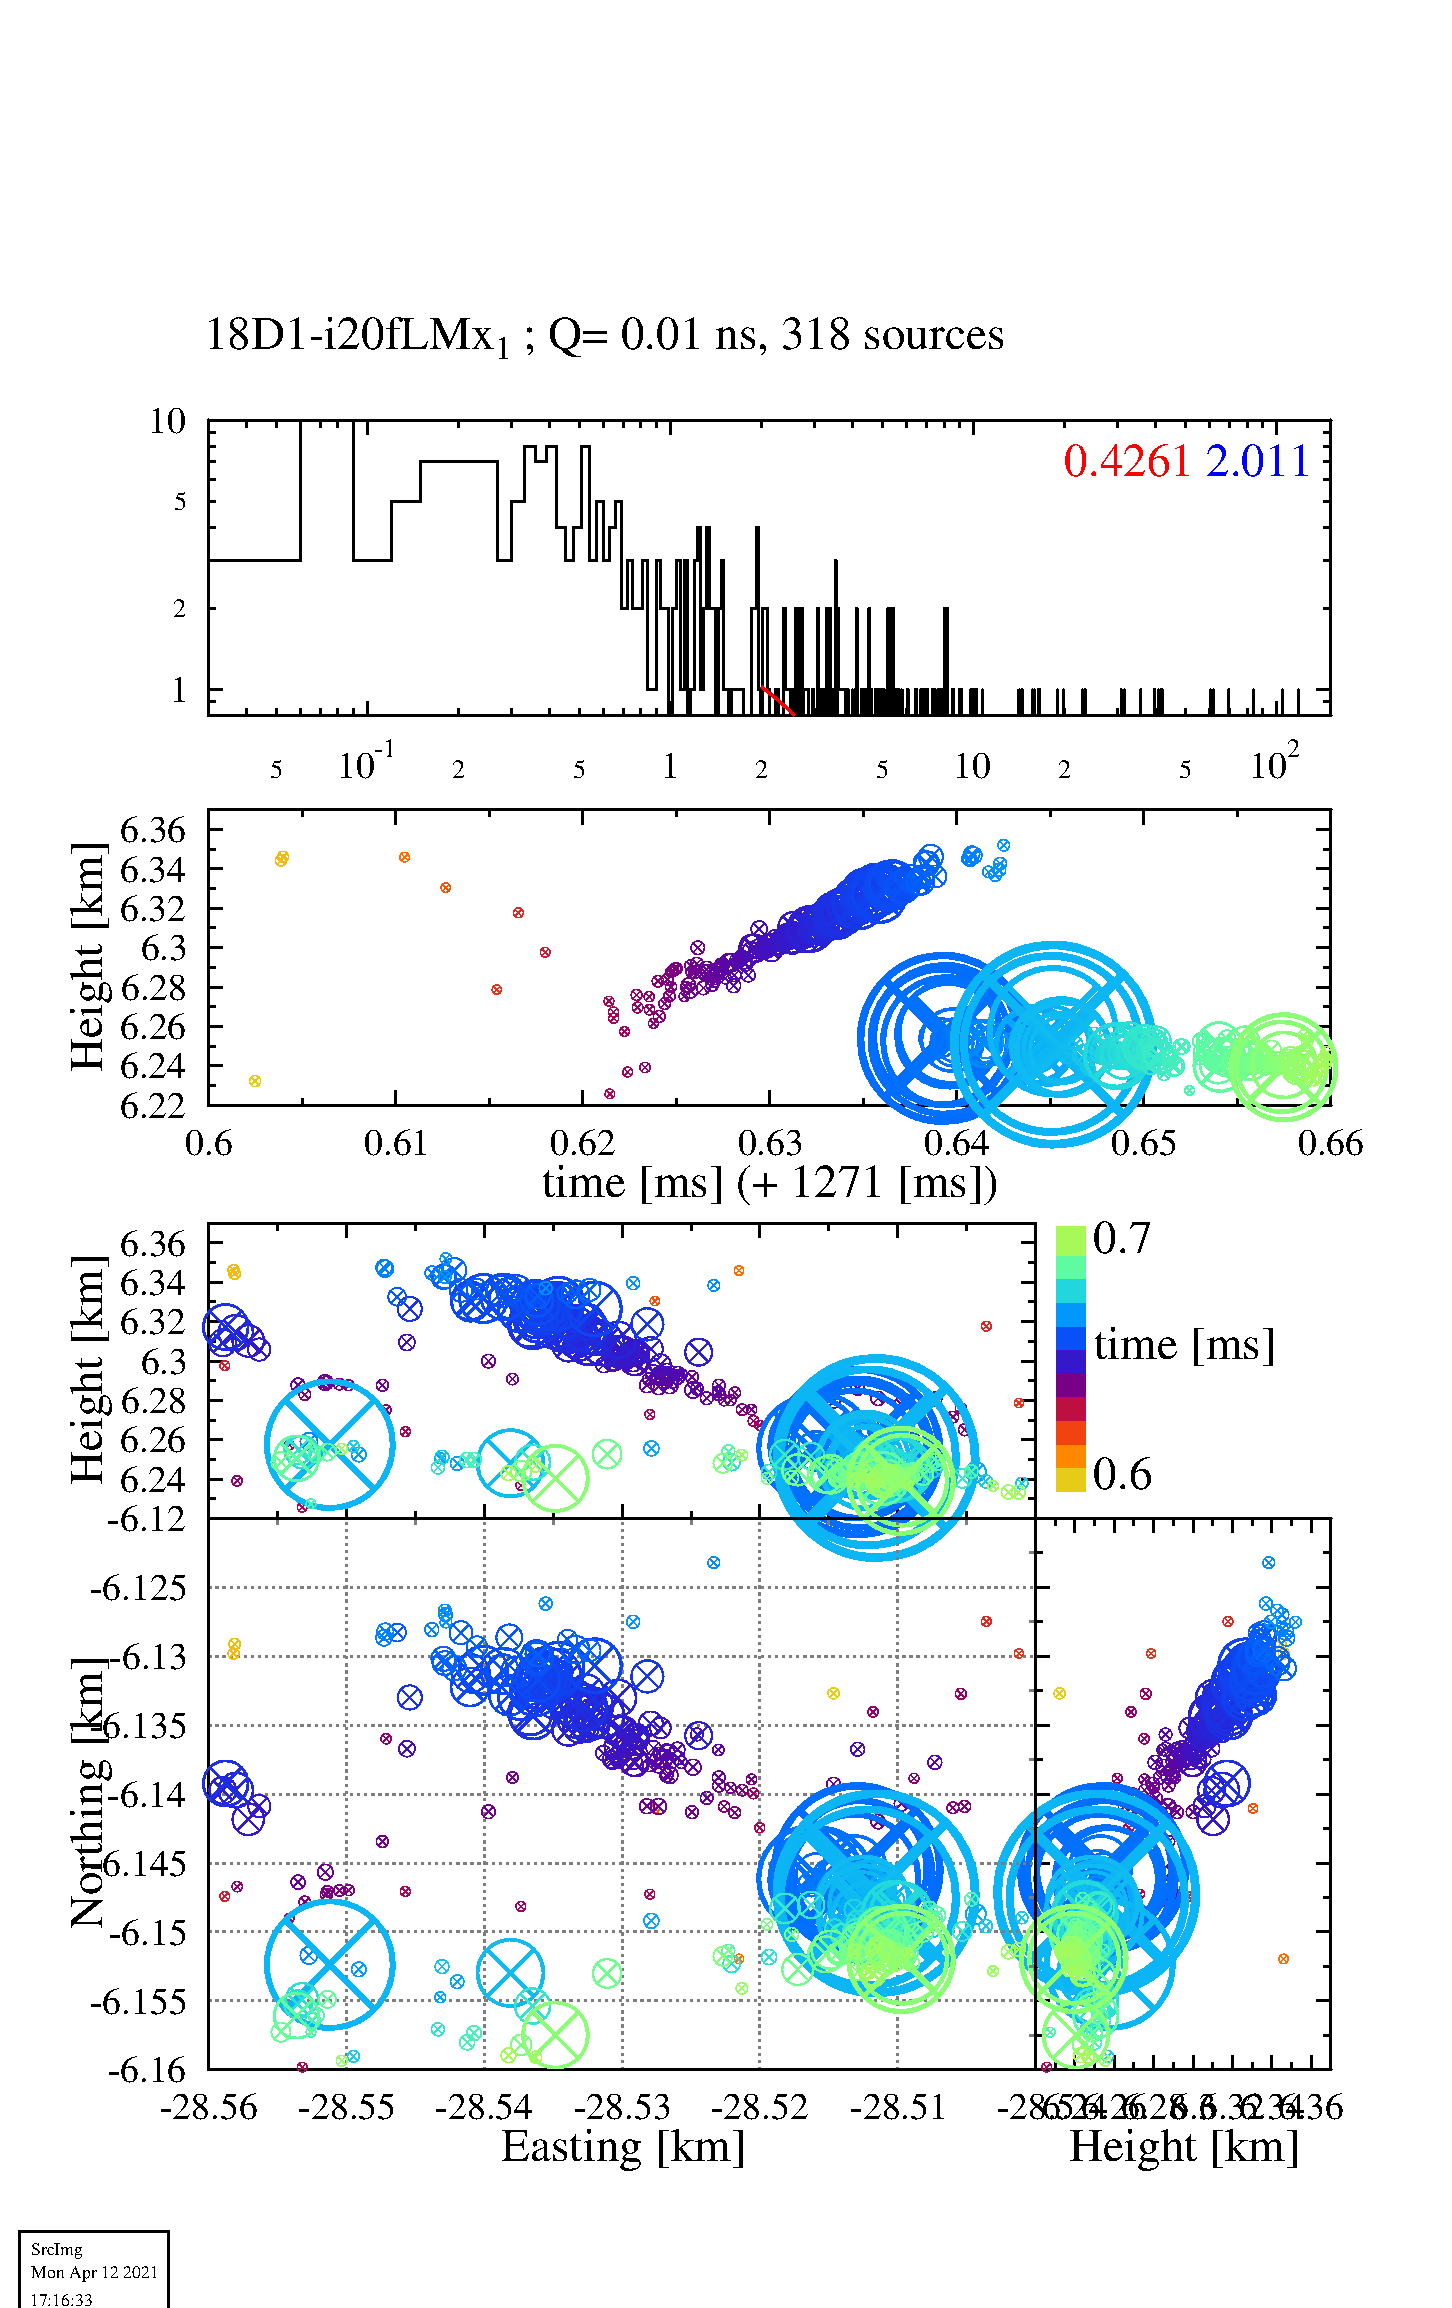
\includegraphics[width=0.49\textwidth]{Figs/18D1-i20fMx_1LIntfSpecSel} }
%\centering{\includegraphics[ bb=1.0cm 2.4cm 24.5cm 25.7cm,clip, width=0.49\textwidth]{../Figs/SE20A7-NPMx_1HIntfSpecSel} }
	\caption{Typical image for the TRID Imager as created by running ``InterfSrcSel.sh".}	 \figlab{TRIDSelSrcsImg}
\end{figure}

The plots will be made for the `Mx' and `Bar' files as well as for X- and Y-dipoles, all resembling \figref{TRIDSelSrcsImg}. This allows for appending seamless the results of different interferometry runs.

} %---------------------------------------------------------------------
